
\def\IosSevenSlider#1#2{
  \tikz[baseline=0.0cm]{
    \coordinate (start) at (0,0);
    \coordinate (end) at (#1,0);
    \coordinate (mark) at ($(start)!#2!(end)$);
    \useasboundingbox (start|- 0,-.25) rectangle (end|- 0, .25);
    \draw[line width=0.4mm, line cap=round, blue!50!cyan] (start) -- (mark) edge[lightgray] (end);
    \node[
      fill=white,
      draw=lightgray,
      very thin,
      blur shadow={
          shadow xshift=0pt,
          shadow opacity=20,
          shadow yshift=-0.9mm,
          shadow blur steps=6,
          shadow blur radius=0.3mm
        },
      circle,
      minimum size=0.25cm,
      inner sep=0pt
    ] at (mark) {};
  }
}
\newcommand{\insertthesisimage}[1]{%
  \includegraphics[height=\smallheight]{assets/general/teaser/#1.png}%
}

%%%%%%%%%%%%%%%%%%%% CoNeRF %%%%%%%%%%%%%%%%%%%%%%
\newcommand{\thesisconerfteasermanual}{
  \def\height{128bp}
  \def\smallheight{64bp}
  \def\sliderwidth{32bp}
  \def\iconsize{6bp}
  \centering

  \tikzsetnextfilename{thesisteaser}
  \tikzset{external/export next=false}
  \resizebox{1.025\linewidth}{!}{
    \begin{tikzpicture}[
        >=stealth',
        overlay/.style={
            anchor=south west,
            draw=black,
            rectangle,
            line width=0pt,
            outer sep=0,
            inner sep=0,
          },
      ]
      \setlength{\fboxsep}{0pt}
      \matrix[
        matrix of nodes,
        column sep=0pt,
        row sep=0pt,
        ampersand replacement=\&,
        inner sep=0,
        outer sep=0
      ] (conerf-pictures) {
        \insertthesisimage{face_1} \&
        \insertthesisimage{face_2} \&
        \insertthesisimage{face_3}    \\
        \insertthesisimage{mask_1} \&
        \insertthesisimage{mask_2} \&
        \insertthesisimage{mask_3}    \\
        \insertthesisimage{depth_1} \&
        \insertthesisimage{depth_2} \&
        \insertthesisimage{depth_3}   \\
        \mbox{\IosSevenSlider{\sliderwidth}{0.0}} \&
        \mbox{\IosSevenSlider{\sliderwidth}{0.0}} \&
        \mbox{\IosSevenSlider{\sliderwidth}{1.0}} \\
        \mbox{\IosSevenSlider{\sliderwidth}{0.0}} \&
        \mbox{\IosSevenSlider{\sliderwidth}{1.0}} \&
        \mbox{\IosSevenSlider{\sliderwidth}{1.0}} \\
        \mbox{\IosSevenSlider{\sliderwidth}{0.0}} \&
        \mbox{\IosSevenSlider{\sliderwidth}{0.5}} \&
        \mbox{\IosSevenSlider{\sliderwidth}{1.0}} \\
      };

      \node[left=0em of conerf-pictures-1-1.west] {\rotatebox{90}{\scriptsize Render}};
      \node[left=0em of conerf-pictures-2-1.west] {\rotatebox{90}{\scriptsize Overlaid Mask}};
      \node[left=-0.2em of conerf-pictures-3-1.west] {\rotatebox{90}{\scriptsize Rendered Depth}};

      \foreach \y in {1,...,3} {
          \node[left=-0.2em of conerf-pictures-4-\y.west] {
\includegraphics[width=\iconsize]{assets/general/teaser/closed-eye.png}};
          \node[right=-0.2em of conerf-pictures-4-\y.east] {
\includegraphics[width=\iconsize]{assets/general/teaser/open-eye.png}};

          \node[left=-0.2em of conerf-pictures-5-\y.west] {
\includegraphics[width=\iconsize]{assets/general/teaser/closed-eye.png}};
          \node[right=-0.2em of conerf-pictures-5-\y.east] {
\includegraphics[width=\iconsize]{assets/general/teaser/open-eye.png}};

          \node[left=-0.2em of conerf-pictures-6-\y.west] {
\includegraphics[width=\iconsize]{assets/general/teaser/frown.png}};
          \node[right=-0.2em of conerf-pictures-6-\y.east] {
\includegraphics[width=\iconsize]{assets/general/teaser/smile.png}};
        }

    \end{tikzpicture}
  }
}

%%%%%%%%%%%%%%%%%%%% BlendFields %%%%%%%%%%%%%%%%%%%%%%
\newcommand{\thesisblendfieldsteasermanual}{
  \tikzsetnextfilename{blendfieldsthesisteaser}
  \tikzset{external/export next=false}
  {
    \centering
    \def\smallheight{64bp}
    \def\sliderwidth{32bp}
    \def\iconsize{6bp}
    \def\blendfieldsdirname{4_blendfields}
    \def\imagewidth{2.3cm}
    \def\imageheight{3.5263671874999996cm}
    \def\smallimagewidth{0.8cm}
    \def\smallimageheight{1.2265625cm}
    \def\borderthickness{0.41pt}
    \def\spysize{24bp}
    \resizebox{\linewidth}{!}{
      \begin{tikzpicture}[
          >=stealth',
          overlay/.style={
              anchor=south west,
              draw=black,
              rectangle,
              line width=0.8pt,
              outer sep=0,
              inner sep=0,
            },
          spy using outlines={
              circle,
              green,
              magnification=3,
              connect spies,
              size=\spysize,
            },
        ]
        \small
        \matrix[matrix of nodes, column sep=1pt, row sep=1pt, ampersand replacement=\&, inner sep=0, outer sep=0] (training) {
          % 
\includegraphics[height=\imageheight]{assets/\blendfieldsdirname/teaser2/ours/0001_mix.png} \&
          % 
\includegraphics[height=\imageheight]{assets/\blendfieldsdirname/teaser2/ours/0003_mix.png} \\
          
\includegraphics[height=\imageheight]{assets/\blendfieldsdirname/teaser2/ours/0004_mix.png} \&
          
\includegraphics[height=\imageheight]{assets/\blendfieldsdirname/teaser2/ours/0003_mix.png} \\
        };
        %   \node[above right=\borderthickness and \borderthickness of training-1-1.south west, overlay]{
        %     
\includegraphics[height=\smallimageheight]{assets/\blendfieldsdirname/teaser2/colorsv2/0001.png}
        %   };
        %   \node[above right=\borderthickness and \borderthickness of training-1-2.south west, overlay]{
        %     
\includegraphics[height=\smallimageheight]{assets/\blendfieldsdirname/teaser2/colorsv2/0002.png}
        %   };
        \node[above right=\borderthickness and \borderthickness of training-1-1.south west, overlay]{
          
\includegraphics[height=\smallimageheight]{assets/\blendfieldsdirname/teaser2/colorsv2/0003.png}
        };
        \node[above right=\borderthickness and \borderthickness of training-1-2.south west, overlay]{
          
\includegraphics[height=\smallimageheight]{assets/\blendfieldsdirname/teaser2/colorsv2/0002.png}
        };

        \matrix[
          matrix of nodes,
          column sep=1pt,
          row sep=1pt,
          ampersand replacement=\&,
          below=0.1em of training,
          inner sep=0,
          outer sep=0
        ] (final) {
          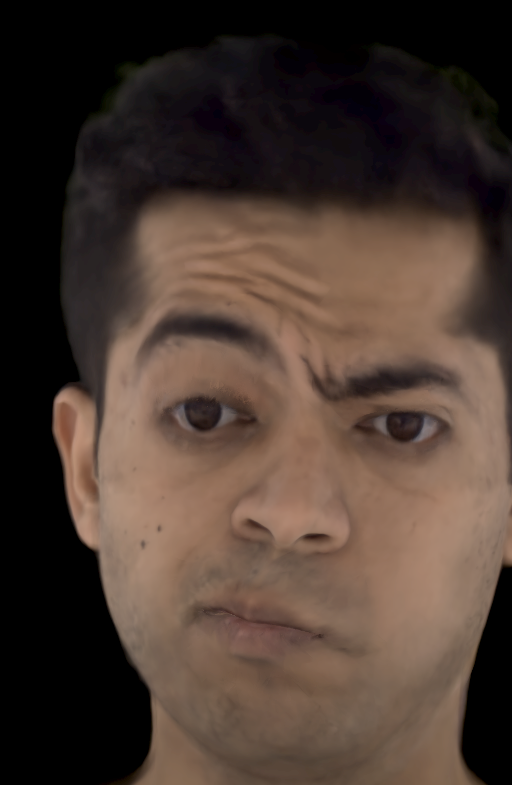
\includegraphics[height=\imageheight]{assets/general/teaser/blendfields-final.png} \\
        };
        \spy[anchor=center,magnification=3,size=32bp] on ([xshift=-0.5em,yshift=1.3em] final-1-1.center) in node[below left=5bp and 5bp] at (final-1-1.north west);

        \spy[anchor=center,magnification=3,size=32bp] on ([xshift=0.5em,yshift=0.2em] final-1-1.center) in node[below right=5bp and 5bp] at (final-1-1.north east);

        \spy[anchor=center,magnification=3,size=32bp] on ([xshift=0em,yshift=-0.3em] final-1-1.center) in node[above left=5bp and 5bp] at (final-1-1.south west);

        \spy[anchor=center,magnification=2,size=32bp] on ([xshift=1.0em,yshift=-1.6em] final-1-1.center) in node[above right=5bp and 5bp] at (final-1-1.south east);

        \node[above right=\borderthickness and \borderthickness of final-1-1.south west, overlay]{
          
\includegraphics[height=\smallimageheight]{assets/\blendfieldsdirname/teaser2/colorsv2/final.png}
        };

        \node[left=3.5em of final-1-1.west, align=center] {\scriptsize \rotatebox{90}{Novel Expression}};
        \node[left=0.5em of training-1-1.west, align=center] {\scriptsize \rotatebox{90}{Reconstructions}};

      \end{tikzpicture}
    }
  }
}

%%%%%%%%%%%%%%%%%%%% Lumigauss %%%%%%%%%%%%%%%%%%%%%%
\newcommand{\thesislumigaussteasermanual}{
  \centering
  \tikzsetnextfilename{lumigauss-thesis-teaser}
  \tikzset{external/export next=false}
  {
    \def\firstrowimageheight{724px}
    \def\secondrowimagewidth{536px}
    \def\imageheight{2cm}
    \resizebox{\linewidth}{!}{
      \begin{tikzpicture}[font=\large]
        \matrix[matrix of nodes, column sep=-0.1pt, row sep=3em, ampersand replacement=\&, inner sep=0, outer sep=0] (training) {
          
\includegraphics[width=\linewidth, trim={50 50 50 225}, clip]{\lumigaussassets/folder_for_kacper/teaser/rec.png} \&
          
\includegraphics[width=\linewidth, trim={50 50 50 225}, clip]{\lumigaussassets/folder_for_kacper/teaser/normals.png}       \\
          
\includegraphics[width=\linewidth, trim={50 0 50 0}, clip]{\lumigaussassets/folder_for_kacper/teaser/env_1_rec.png} \&
          
\includegraphics[width=\linewidth, trim={50 0 50 0}, clip]{\lumigaussassets/folder_for_kacper/teaser/env_1_shadows.png} \\
        };
        \def\fontscale{1.5}

        \node[above=0.5em of training-1-1.north, anchor=base,scale=\fontscale] {Reconstruction};
        \node[above=0.5em of training-1-2.north, anchor=base,scale=\fontscale] {Rendered Normals};

        \node[above=0.5em of training-2-1.north, anchor=base,scale=\fontscale] {Novel Light};
        \node[above=0.5em of training-2-2.north, anchor=base,scale=\fontscale] {Predicted Shadows};

        \node[below left=2em and 0.1pt of training-2-1.north east, anchor=center]{
\includegraphics[width=4em]{\lumigaussassets/folder_for_kacper/teaser/env_1_map.png}};
      \end{tikzpicture}
    }
  }
}

%%%%%%%%%%%%%%%%%%%% CLoG %%%%%%%%%%%%%%%%%%%%%%
\newcommand{\insertsmallteaser}[1]{
  \includegraphics[height=\height, trim={14em 2em 14em 0}, clip]{assets/\clogdirname/teaser/teaser_scale=#1.png}
}
\newcommand{\insertsmalluv}[1]{
  \includegraphics[height=\smallheightuv]{assets/\clogdirname/teaser/uv_scale=#1.png}
}
\newcommand{\thesisclogteasermanual}{
  \def\height{128bp}
  \def\smallheight{64bp}
  \def\smallheightuv{76bp}
  \centering

  \tikzsetnextfilename{thesisclogteaser}
  \tikzset{external/export next=false}
  \resizebox{\linewidth}{!}{
    \begin{tikzpicture}[
        >=stealth',
        overlay/.style={
            anchor=south west,
            draw=black,
            rectangle,
            line width=0pt,
            outer sep=0,
            inner sep=0,
          },
      ]
      \begin{scope}[xshift=3em]
        \node (representation) {
\includegraphics[height=\height, trim={12em 2em 12em 0}, clip]{assets/\clogdirname/teaser/teaser_1_blended.png}};
        \node[circle, thick, fill=white, draw, below left=4.5em and 1.25em of representation.south] (x1) {};
        \node[circle, thick, fill=white, draw, below=0.1em of x1] (x2) {};
        \node[circle, thick, fill=white, draw, below=0.1em of x2] (x3) {};
        \node[circle, thick, fill=white, draw, above=0.1em of x1] (x4) {};
        \node[circle, thick, fill=white, draw, above=0.1em of x4] (x5) {};

        \node[circle, thick, fill=white, draw, right=2em of x1] (x11) {};
        \node[circle, thick, fill=white, draw, below=0.1em of x11] (x12) {};
        \node[circle, thick, fill=white, draw, above=0.1em of x11] (x13) {};

        \foreach \x in {1,...,5}
        \foreach \y in {1,...,3}
        \draw (x\x) -- (x1\y);
        \matrix[
          matrix of nodes,
          right=1em of representation,
          column sep=0pt,
          row sep=0pt,
          ampersand replacement=\&,
          inner sep=0,
          outer sep=0
        ] (pictures) {
          \insertsmallteaser{0.1} \&
          \insertsmallteaser{1.0} \\
        };

        \node[below=1em of pictures-1-1.south, outer sep=2pt] (uv1) {\insertsmalluv{0.1}};
        \node[below=1em of pictures-1-2.south, outer sep=2pt] (uv2) {\insertsmalluv{1.0}};
        \draw[-stealth, shorten <=2pt, decoration={snake}, decorate, thick] (x11) --  (uv1);

        \node[above=-0.6em of representation, anchor=base, align=center] {Representation};

        \node[above=-0.3em of pictures, anchor=base, align=center] (novelview) {Novel View and LoD Synthesis};

        \node[below=0em of pictures, align=center] {Learned 2D Grid of Features};

        \draw[-stealth,  thick, dashed, ->] (uv1.south west) -- node [below, midway] {Increasing Continuous LoD} (uv2.south east);

        \node[below=0.5em of representation.south] {Modulator};
      \end{scope}

    \end{tikzpicture}
  }
}

\newcommand{\thesisteaserfigure}{
  \begin{figure}
    \label{fig:thesis-teaser}
    \hspace{-2em}
    \centering
    \begin{subfigure}[b]{0.54\linewidth}
      \centering
      \thesisconerfteasermanual
      \caption{\conerf{} -- control with sparse annotations}
      \label{subfig:conerf-teaser}
    \end{subfigure}
    \hfill{}
    \begin{subfigure}[b]{0.453\linewidth}
      \centering
      \thesisblendfieldsteasermanual
      \caption{\blendfields{} -- control with physical features}
      \label{subfig:blendfields-teaser}
    \end{subfigure}
    \\[1.5em]
    \begin{subfigure}[b]{0.455\linewidth}
      \centering
      \thesislumigaussteasermanual
      \caption{\lumigauss{} -- control with physical constraints}
      \label{subfig:lumigauss-teaser}
    \end{subfigure}
    \hfill{}
    \begin{subfigure}[b]{0.525\linewidth}
      \centering
      \thesisclogteasermanual
      \caption{\clog{} -- control with structural constraints}
      \label{subfig:clog-teaser}
    \end{subfigure}
    \hspace{-1.4em}
    \caption[Teaser introducing works included in this thesis]{
      \textbf{Teaser} -- This thesis introduces a series of publications that advance the state-of-the-art in controllable radiance field methods.
      We present the following papers: \conerf~\cite{kania2022conerf}
      in~\cref{subfig:conerf-teaser}, \blendfields~\cite{kania2023blendfields}
      in~\cref{subfig:blendfields-teaser}, \lumigauss~\cite{kaleta2024lumigauss}
      in~\cref{subfig:lumigauss-teaser} and \clog~in~\cref{subfig:clog-teaser}.
      Together, these complementary approaches enable unprecedented control over 3D
      content through sparse annotations (\conerf{} and \blendfields{}), dynamic
      environment lighting (\lumigauss{}), and optimized computational efficiency
      for single-image rendering (\clog{}), addressing key challenges in modern
      neural rendering systems.
    }
  \end{figure}

}